% IEEE/IFIP NOMS 2027 submission. Full paper: 8 pages main text + references/appendix, 12 pages max.
% All tables are generated from results JSON by make_tables.py; numbers in the prose are listed in tables/numbers.json.
\documentclass[conference]{IEEEtran}
\usepackage[T1]{fontenc}
\usepackage{amsmath,amssymb}
\usepackage{graphicx}
\usepackage{booktabs}
\usepackage{url}
\usepackage{xcolor}
\usepackage{stfloats}
\usepackage[hidelinks]{hyperref}
\graphicspath{{figures/}}
\newcommand{\dg}{$^\dagger$}

\begin{document}

\title{Will It Catch Tomorrow's Attack? How Operators Should Evaluate Learned Network Intrusion Detectors Before Trusting Them on Zero-Day Traffic}

% Single-blind review: the author list must match the EDAS registration exactly.
\author{\IEEEauthorblockN{Hafsa [surname]\IEEEauthorrefmark{1}, [co-authors]}
\IEEEauthorblockA{\IEEEauthorrefmark{1}[Department, University, City, Country]\\ Email: [email]}}

\maketitle

\begin{abstract}
Operators deploy learned network intrusion detection systems (NIDS) to catch attacks that did not exist at training time, yet they choose detectors using a laboratory protocol: one attack class is held out of a randomly split benchmark (LOACO). We ask whether that protocol tells an operator what will happen when a new attack class actually arrives later in time, together with drifting benign traffic. We build a pre-registered, leakage-controlled benchmark on four NetFlow-v3 datasets and LYCOS-IDS2017, with grouped and temporal splits and deduplicated flow windows, and evaluate 12 detectors from five families over five seeds. On day-scheduled captures, LOACO under a temporal split has zero feasible folds on two of three datasets, while natural temporal novelty remains available. The best detector family changes with dataset and protocol, and a plain XGBoost classifier matches or beats the leading novelty family in four of seven evaluations. Natural novelty raises the seed variability of every supervised score by 1.7--17$\times$, which LOACO hides, and max-softmax and energy scores fall below chance because confidently detected attacks read as normal. We turn these findings into an evaluation checklist for operators and release all splits, code and amendments.
\end{abstract}

\begin{IEEEkeywords}
network intrusion detection, zero-day attacks, network security management, out-of-distribution detection, evaluation methodology, NetFlow
\end{IEEEkeywords}

\section{Introduction}
A network operator who deploys a learned NIDS is buying protection against attacks that are not in its training data. Before trusting it, the operator needs evidence that the detector flags a new attack class when that class first appears in the network. In practice that evidence comes from a laboratory protocol, leave-one-attack-class-out (LOACO): one class is removed from training and the detector must flag it at test time~\cite{wilkie2026,jodayree2026,sarhan2023zeroday}. This paper asks whether that evidence transfers to operations.

The question matters because LOACO and deployment differ. LOACO removes a class artificially from a randomly split capture, so benign traffic at test time comes from the same hours as training. In operation, a new class arrives later in time, together with drifting benign traffic, new hosts and new tools. Sommer and Paxson warned that anomaly detection outside a closed world is harder than benchmarks suggest~\cite{sommer2010}, and later work showed that sampling bias, data snooping and weak baselines inflate security-ML results~\cite{arp2022,apruzzese2023,engelen2021}. Two practices widen the gap further: many NIDS papers score novelty with confidence scores designed for multi-class image recognition, such as maximum softmax probability (MSP)~\cite{hendrycks2017} or energy~\cite{liu2020energy}, and few report seed variability or pre-register their hypotheses~\cite{nosek2018}.

We compare LOACO with \emph{natural temporal novelty}, in which attack classes appear only after the training period, on the same detectors and data. Our benchmark covers five public datasets, 12 detectors in five families and five seeds per configuration; every number comes from one code commit and is regenerated from stored result files. From the operator's point of view, the results give six lessons:
\begin{itemize}
\item \textbf{C1 Feasibility.} On day-scheduled captures, temporal LOACO has zero feasible folds on CIC-IDS2018 and ToN-IoT and one on LYCOS-IDS2017 under a purged block split, while natural novelty offers 2--5 evaluable classes per dataset.
\item \textbf{C2 No family dominates.} The best family changes with dataset and protocol, and XGBoost matches or beats the leading novelty family in four of seven evaluations.
\item \textbf{C3 Hidden instability.} Natural novelty raises the seed standard deviation of every supervised score 1.7--17$\times$ over LOACO; seeded benign-only detectors stay stable.
\item \textbf{C4 Score validity.} MSP and energy fall below chance in binary NIDS; the classifier's attack probability does not on average.
\item \textbf{C5 Generalization.} Temporal-split effects are dataset-specific, and 67\% of 108 zero-shot cross-dataset cells fall between 0.3 and 0.6 AUC.
\item \textbf{C6 Negative results and release.} Four pre-registered hypotheses failed their frozen gates; we report them and release splits, amendments and provenance.
\end{itemize}
Section~\ref{sec:bg} defines the protocols and scores, Section~\ref{sec:method} the benchmark, Section~\ref{sec:setup} the setup, Section~\ref{sec:results} the results and Section~\ref{sec:disc} the operator checklist and limitations.

\section{Background and Related Work}\label{sec:bg}
\subsection{Zero-day evaluation protocols}
\emph{LOACO} removes one attack class from the training pool; the test set holds benign windows plus that class. Splits are usually random; we group by 1-hour blocks. \emph{Natural temporal novelty} splits flows in time; classes that occur only after the training period are unseen by construction, and benign traffic drifts as it would in operation. \emph{Purged block LOACO}, for short captures, assigns short time blocks to splits within each day and drops blocks adjacent to test or validation blocks, following purged cross-validation~\cite{lopezdeprado2018}. LOACO asks whether a detector generalizes to a missing class under the training distribution; natural novelty asks it under real temporal shift.

\subsection{Novelty scores and the binary pitfall}
Out-of-distribution (OOD) detection assigns each input a score that should be higher for inputs unlike the training data~\cite{yang2024ood}. We group scores into families by what they read: \emph{classifier-confidence} scores use the output layer (MSP~\cite{hendrycks2017}, energy~\cite{liu2020energy}, the attack probability P(attack)); \emph{representation-distance} scores use hidden features (Mahalanobis~\cite{lee2018}, $k$-nearest-neighbour~\cite{sun2022knn}, and the deviation of a recurrent state from a benign reference); \emph{benign-only} detectors never see attacks~\cite{liu2008if,scholkopf2001,mirsky2018}; \emph{contrastive} detectors such as CLAD~\cite{wilkie2026} train an embedding with benign and known attacks. MSP and energy measure how sure a classifier is, not which class it chose. In a two-class NIDS a new attack that is confidently classified as \emph{attack} has high MSP and therefore reads as in-distribution: the expected outcome of successful detection becomes a missed novelty.

\subsection{Related work}
Zero-day NIDS work evaluates under class hold-out: Sarhan et al. framed it as zero-shot learning and linked low detection to large Wasserstein distance from known attacks~\cite{sarhan2023zeroday}; Zoppi et al. compared 47 algorithms on unknown attacks and found unsupervised meta-learners strongest~\cite{zoppi2023}; Wilkie et al. proposed CLAD and reported gains on held-out LYCOS-IDS2017 classes~\cite{wilkie2026}; Jodayree et al. reported an AUROC-OOD of 0.975 under leave-one-attack-out on IoMT traffic~\cite{jodayree2026}. Flow-based NIDS on these NetFlow datasets are commonly evaluated in-distribution, e.g.\ the graph-based E-GraphSAGE~\cite{lo2022egraphsage}; cross-dataset studies report sharp drops outside the training domain~\cite{layeghy2023xdomain,layeghy2023dinids,martinez2026}. None compares hold-out with natural temporal novelty on the same detectors, reports per-class seed variability, or pre-registers its hypotheses. Appendix~\ref{app:related} extends this review and positions the paper against prior work.

\section{Benchmark Design}\label{sec:method}
The benchmark fixes data, splits, backbone and detectors in advance; every protocol change was recorded as a dated, hashed amendment before the runs it governs.

\subsection{Datasets}
All datasets are public and were downloaded from official sources; each archive's SHA-256, row count and column list is recorded in a manifest. D1--D4 are the NetFlow-v3 versions~\cite{luay2025} of CSE-CIC-IDS2018~\cite{sharafaldin2018}, UNSW-NB15~\cite{moustafa2015}, ToN-IoT~\cite{moustafa2021} and BoT-IoT~\cite{koroniotis2019}, sharing a 53-feature schema~\cite{sarhan2021netflow,sarhan2022standard}. D5 is LYCOS-IDS2017~\cite{rosay2021}, a corrected CIC-IDS2017, processed in its own 73-feature space and not used for transfer (Table~\ref{tab:datasets}). D4 has only 1,315 benign windows, too few for its own splits, so it serves only as a transfer target. D1's 14 attack labels map exactly to six families; LOACO on D1 holds out families, so a held-out class has no near-identical sibling in training.

% generated by paper/noms2027/make_tables.py from results JSON; do not edit
\begin{table}[t]
\centering\scriptsize\setlength{\tabcolsep}{1.8pt}
\caption{Datasets. Windows are counted after global deduplication.}\label{tab:datasets}
\begin{tabular}{llrrrl}
\toprule
ID & Dataset & Flows & Windows & Att.\ cl. & Role \\
\midrule
D1 & NF-CSE-CIC-IDS2018-v3 & 20,115,529 & 1,255,180 & 14 & LOACO, NN, transfer \\
D2 & NF-UNSW-NB15-v3 & 2,365,424 & 147,801 & 9 & LOACO, transfer \\
D3 & NF-ToN-IoT-v3 & 27,520,260 & 1,553,191 & 9 & LOACO, NN, transfer \\
D4 & NF-BoT-IoT-v3 & 16,933,808 & 890,852 & 4 & transfer target \\
D5 & LYCOS-IDS2017 & 1,837,498 & 114,783 & 13 & NN, purged LOACO \\
\bottomrule
\end{tabular}
\end{table}


\subsection{Preprocessing and leakage control}
Identifier columns (addresses, ports, DNS query ID) are dropped and timestamps are used only for ordering and splitting. Minimum and maximum TTL are dropped as a known label-leakage artifact. Infinite values are imputed with the training median, non-negative heavy-tailed counts are transformed with $\log(1+x)$, and features are standardized with training statistics; zero-variance features and one of each pair with $|r|\geq0.999999$ are removed, leaving 41 common features for D1--D4. Flows are sorted by start time and grouped into 1-hour blocks (10-minute blocks for D5's purged split). Windows of $T{=}32$ consecutive flows with stride 16 never cross a block boundary; a window is labelled attack if any flow is an attack, and its class is the majority attack class. Windows are hashed and exact duplicates removed globally (9.7\% of D3 and 15.8\% of D4 windows). Every stage runs fail-closed integrity checks (row and block disjointness across splits, dedup, balance, feature lists): 538 checks at preprocessing for D1--D4 and further checks for each derived split (e.g., 32 for D5's purged split); all passed.

\subsection{Splits and zero-day protocols}
\emph{grouped\_random} shuffles blocks into 60/20/20 train/validation/test; \emph{temporal\_gap} orders blocks in time, takes the first 60\% for training, discards one gap block, then 20\% validation and 20\% test. \emph{LOACO} uses grouped\_random: a class is held out if it has at least 200 training-pool windows (by majority label) and at least one test window; training and validation exclude every window containing any flow of the held-out class. In practice every fold has at least 81 held-out test windows. \emph{Natural novelty} uses temporal\_gap: classes that occur in the test period but not in the training period are scored as unseen; validation is the last 20\% of the training period (train-tail validation), because on D1 every temporal validation window contains a natural-novelty flow. \emph{Purged block} (D5 only) splits 10-minute blocks 60/20/20 within each capture day, removes train and validation blocks adjacent to a test block and train blocks adjacent to a validation block~\cite{lopezdeprado2018}; for this split a held-out class also needs at least 50 test windows. Training sets are balanced 1:1 (7,000 benign and 7,000 attack windows); validation and test sets use a 5:1 benign-to-attack ratio, capped at 2,500 benign and 500 attack windows.

\subsection{Backbone}
All supervised scores are read from one recurrent backbone, the fixed-equilibrium variant of a homeostatic sequence detector. Each flow vector is embedded as $z_t=\mathrm{LayerNorm}(W x_t)\in\mathbb{R}^{128}$. A state $h_t$, initialised at a benign reference $E$, tracks the input through per-step, per-channel gates:
\begin{align*}
h_t &= h_{t-1} + \alpha_t\odot(z_t-E) - \beta_t\odot(h_{t-1}-E),\\
[\alpha_t,\beta_t] &= \sigma\big(W_g[z_t,h_{t-1}]\big).
\end{align*}
$E$ is not learned: it is the mean embedding of benign training windows (tracked by an exponential moving average during training and set exactly afterwards) and stays fixed within a window. Homeostatic \emph{stress} is $\frac{1}{TD}\sum_{t,d}|h_{t,d}-E_d|$. A two-layer MLP head (linear--GELU--linear) reads $[h_T,\ \frac{1}{T}\sum_t h_t,\ \text{stress}]$ and outputs two logits; its hidden layer is the penultimate representation. We chose this backbone because it exposes a representation-distance score inside the model; other neural backbones were not built (Section~\ref{sec:limits}).

\subsection{Detectors}
\emph{Confidence:} MSP ($1-\max$ softmax), energy (negative log-sum-exp of logits) and P(attack), the softmax attack probability. \emph{Representation:} stress; Mahalanobis distance to a Ledoit--Wolf Gaussian fitted on benign penultimate features~\cite{lee2018}; distance to the 10th benign nearest neighbour of $\ell_2$-normalised penultimate features~\cite{sun2022knn}. \emph{Benign-only}, fitted on benign training windows: Isolation Forest (200 trees)~\cite{liu2008if}, one-class SVM (RBF, $\nu{=}0.1$)~\cite{scholkopf2001}, PCA reconstruction error (95\% variance) and an autoencoder. \emph{Contrastive:} CLAD~\cite{wilkie2026}, implemented from its paper with open details fixed before training. \emph{Supervised reference:} XGBoost~\cite{chen2016xgb} on flattened windows, 300 trees, depth 6, learning rate 0.1. Higher scores always mean more anomalous; orientation was fixed before any run. P(attack) was added after the last confirmatory gate (marked \dg), when the confidence-score flaw in Section~\ref{sec:c4} was recorded.

\subsection{Pre-registration and provenance}
Research questions, metrics and gates were written to a file and hashed before each experiment, and every result records that hash, the code commit and the dataset hashes. Six dated, hashed amendments changed the plan, each before the runs it governs: two because data counts made a frozen rule infeasible (an empty validation split; zero LOACO folds on D5), three that set a new direction after a gate returned STOP, and one that added P(attack) and the family split after the last gate. Four confirmatory gates were evaluated exactly as frozen; all returned STOP (Section~\ref{sec:c6}). The final benchmark is descriptive: it applies no thresholds and reports intervals, not tests.

\section{Experimental Setup}\label{sec:setup}
\emph{Training.} The backbone uses AdamW (learning rate $10^{-3}$, weight decay $10^{-4}$), cosine annealing, gradient clipping at 1.0, batch 256 and 15 epochs, with no per-detector tuning. The checkpoint with the best validation macro-F1 is primary (CLAD: best validation AUROC). The final-epoch state of the same training run is kept and scored as a sensitivity analysis. XGBoost's subsampling is fixed at 1, which makes it deterministic.
\emph{Statistics.} Seeds are 17, 23, 42, 101 and 202; a seeding regression test runs before every experiment. Per detector and class we report ROC AUC as the mean over seeds with a Student-$t$ 95\% interval ($t{=}2.776$), the seed standard deviation and the fraction of seeds below 0.5. Family means average the family's detectors and the evaluation's classes, with a 95\% bootstrap interval resampling classes and seeds independently (2,000 resamples).
\emph{Evaluations.} LOACO on D1 families, D2 and D3 (6, 8, 6 folds); natural novelty on D1, D3, D5 (2, 5, 2 classes); purged LOACO on D5 (1 fold); in-distribution detection on D1, D2, D3, D5 under both splits; zero-shot transfer from D1--D3 to all other NetFlow-v3 datasets (9 pairs).
\emph{Compute and provenance.} All 160 final runs used one code commit and ran on a CPU-only cloud container (4 vCPUs, Intel Xeon at 2.10\,GHz, no GPU); together they took 4.27\,h of wall-clock time (96\,s per run on average). The report script refuses to run if commits differ within an experiment; one run interrupted by a container restart was resumed from the same commit.

\section{Results}\label{sec:results}
All values are mean AUC over five seeds; brackets are 95\% intervals.

\subsection{C1: Hold-out is often infeasible on time-ordered captures}
% generated by paper/noms2027/make_tables.py from results JSON; do not edit
\begin{table}[t]
\centering\scriptsize
\caption{Protocol feasibility: feasible LOACO folds per split and natural-novelty (NN) classes.}\label{tab:feasibility}
\begin{tabular}{lccc}
\toprule
Dataset & LOACO, grouped & LOACO, temporal & NN classes \\
\midrule
D1 & 6 (fam.) & 0 & 2 \\
D2 & 8 & 8 & 0 \\
D3 & 6 & 0 & 5 \\
D5 & 0 & 0 & 2 \\
\midrule
D5 purged block & \multicolumn{2}{c}{1 (dos\_hulk)} & -- \\
\bottomrule
\end{tabular}
\end{table}

Temporal LOACO is infeasible on two of three day-scheduled captures, while natural novelty is available on all three (Table~\ref{tab:feasibility}). In D1 and D3 the time-ordered split puts every attack class wholly in the training period or wholly in the test period (D1: 12 and 2 of 14 classes; D3: 4 and 5 of 9), so no class can be held out from a training pool that contains it. D2 interleaves attacks over time and supports LOACO under both splits, but has no test-only classes. On D5 the purged 10-minute split kept 125 of 219 blocks and yielded one feasible fold (dos\_hulk); the other twelve classes either fell wholly outside the test split or had fewer than 200 training windows (web brute force had 199). \textbf{Operator lesson:} on realistic, time-ordered captures, natural novelty is often the only zero-day evaluation available.

\subsection{C2: No detector family dominates}
% generated by paper/noms2027/make_tables.py from results JSON; do not edit
\begin{table}[t]
\centering\scriptsize\setlength{\tabcolsep}{2.6pt}
\caption{Family mean AUC (5 seeds). Bold: leading novelty family. Underlined: XGBoost $\geq$ leading novelty family. Conf.\ = MSP, Energy, P(attack); Repr.\ = stress, Mahalanobis, kNN; Benign = IF, OCSVM, PCA, AE.}\label{tab:families}
\begin{tabular}{lcccccc}
\toprule
Evaluation & Cl. & Conf. & Repr. & Benign & CLAD & XGB \\
\midrule
LOACO D1 (families) & 6 & 0.553 & \textbf{0.729} & 0.660 & 0.653 & 0.682 \\
LOACO D2 & 8 & 0.439 & \textbf{0.977} & 0.807 & 0.949 & \underline{0.998} \\
LOACO D3 & 6 & 0.426 & 0.881 & \textbf{0.903} & 0.780 & 0.862 \\
Purged LOACO D5 & 1 & 0.580 & \textbf{0.998} & 0.833 & 0.972 & \underline{1.000} \\
Natural nov.\ D1 & 2 & 0.529 & \textbf{0.623} & 0.505 & 0.574 & 0.523 \\
Natural nov.\ D3 & 5 & 0.467 & 0.522 & \textbf{0.898} & 0.823 & \underline{0.923} \\
Natural nov.\ D5 & 2 & 0.256 & \textbf{0.940} & 0.794 & 0.864 & \underline{0.968} \\
\bottomrule
\end{tabular}
\end{table}

The leading novelty family changes across evaluations (Table~\ref{tab:families}, Fig.~\ref{fig:heatmap}): representation-distance scores lead in five evaluations and benign-only detectors in two. The largest reversal is on D3. Under LOACO, benign-only and representation scores are close (benign-only minus representation $+0.022$ [$+0.004$, $+0.047$]); under natural novelty, benign-only detectors lead by $+0.376$ [$+0.247$, $+0.500$], and the representation family is at chance in the mean (0.522 [0.402, 0.647]). Under natural novelty on D1 every family is weak; the best is representation at 0.623 [0.562, 0.692]. CLAD never leads: it trails benign-only detectors on LOACO D3 ($-0.123$ [$-0.277$, $-0.034$]) and natural novelty D3 ($-0.075$ [$-0.130$, $-0.023$]), is below 0.5 on every seed for D3 LOACO ddos (0.372), and beats benign-only detectors on LOACO D2 ($+0.142$ [$+0.119$, $+0.164$]). XGBoost exceeds the leading novelty family on LOACO D2 (0.998 vs 0.977), natural novelty D3 (0.923 vs 0.898) and natural novelty D5 (0.968 vs 0.940), and ties it on purged D5. \textbf{Operator lesson:} a detector chosen under one protocol may be the wrong choice under another, and a plain supervised classifier is a necessary baseline.

\begin{figure*}[t]
\centering
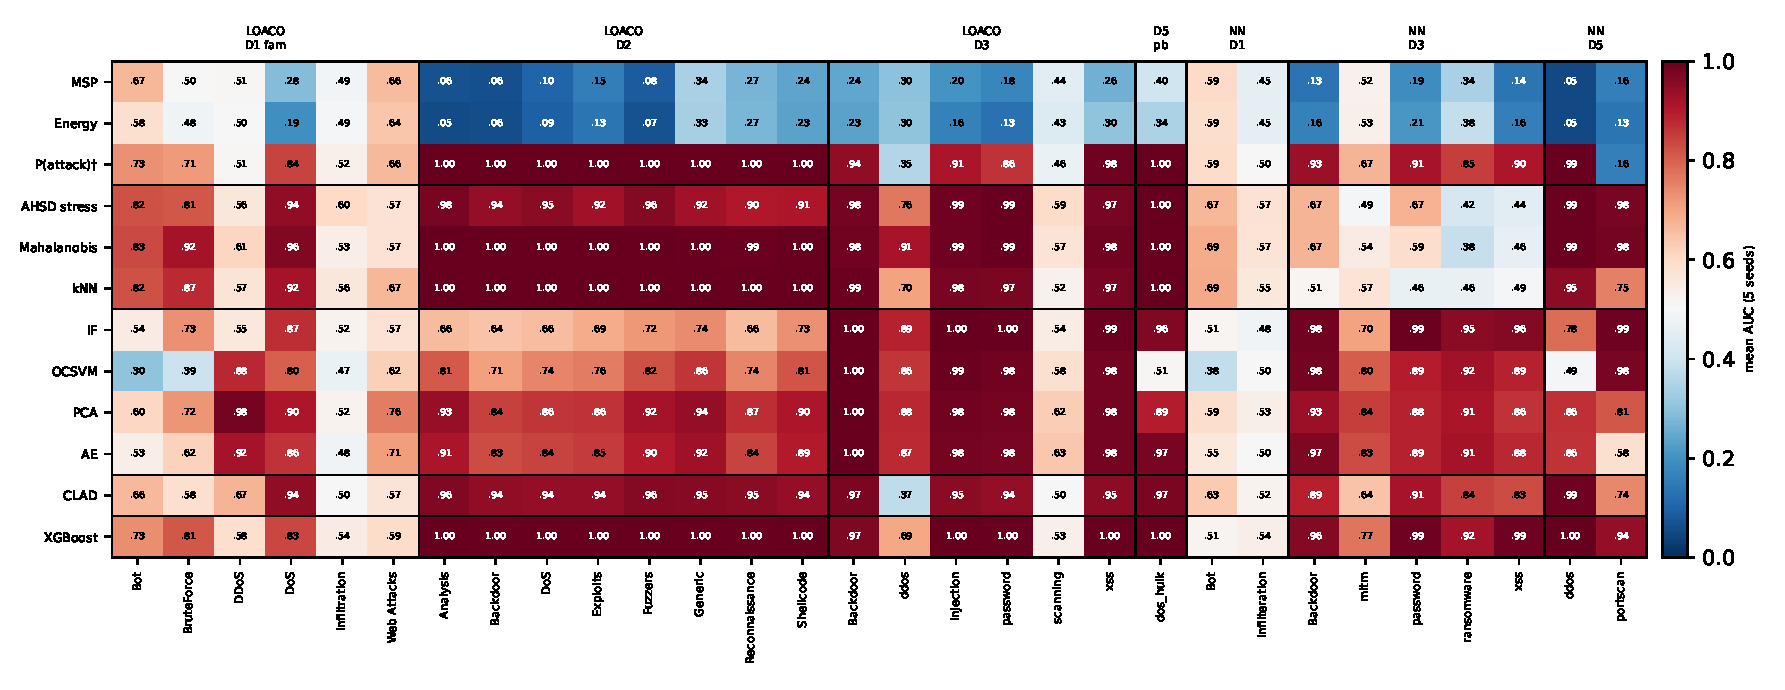
\includegraphics[width=\textwidth]{F3_auc_heatmap}
\caption{Mean AUC per detector (rows, grouped by family) and class (columns, grouped by protocol and dataset). Red $>0.5$, blue $<0.5$.}
\label{fig:heatmap}
\end{figure*}

\subsection{C3: Natural novelty exposes instability that LOACO hides}
% generated by paper/noms2027/make_tables.py from results JSON; do not edit
\begin{table}[t]
\centering\scriptsize
\caption{Mean seed std of AUC over classes: LOACO (D1 families, D2, D3) vs natural novelty (D1, D3, D5). OCSVM, PCA and XGBoost are deterministic (std 0) and omitted.}\label{tab:seedstd}
\begin{tabular}{lccc}
\toprule
Detector & LOACO & Natural nov. & Ratio \\
\midrule
MSP & 0.061 & 0.103 & 1.7$\times$ \\
Energy & 0.055 & 0.100 & 1.8$\times$ \\
P(attack)$^\dagger$ & 0.042 & 0.082 & 2.0$\times$ \\
Stress & 0.019 & 0.110 & 5.8$\times$ \\
Mahalanobis & 0.009 & 0.074 & 7.9$\times$ \\
kNN & 0.013 & 0.215 & 17.0$\times$ \\
CLAD & 0.020 & 0.058 & 2.9$\times$ \\
IF & 0.007 & 0.008 & 1.1$\times$ \\
AE & 0.002 & 0.017 & 9.2$\times$ \\
\bottomrule
\end{tabular}
\end{table}

Every supervised score is less stable under natural novelty than under LOACO (Table~\ref{tab:seedstd}, Fig.~\ref{fig:seedstd}), by 1.7$\times$ (MSP) to 17$\times$ (kNN). The two seeded benign-only detectors stay below 0.018, below every supervised score's minimum of 0.074; the autoencoder's large ratio comes from a near-zero LOACO baseline and one class (D5 portscan). On D3 natural novelty, kNN has a seed standard deviation of 0.33--0.40 AUC on four of five classes: the same detector can rank first or last depending on the seed. \textbf{Operator lesson:} a single training run says little about a supervised detector's zero-day behaviour; evaluate several seeds under natural novelty.

\begin{figure}[t]
\centering
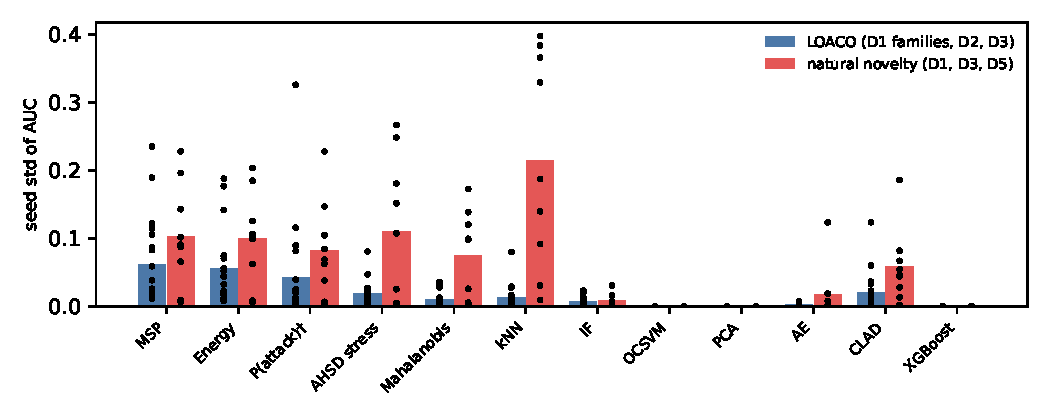
\includegraphics[width=\columnwidth]{F4_seed_std}
\caption{Seed standard deviation of AUC per detector; bars are means over classes, dots individual classes.}
\label{fig:seedstd}
\end{figure}

\subsection{C4: Confidence-magnitude scores are invalid in binary NIDS}\label{sec:c4}
% generated by paper/noms2027/make_tables.py from results JSON; do not edit
\begin{table}[t]
\centering\scriptsize
\caption{Confidence-magnitude scores vs the attack probability and representation distance (mean AUC over classes).}\label{tab:confidence}
\begin{tabular}{lcccc}
\toprule
Evaluation & MSP & Energy & P(attack)$^\dagger$ & Repr. \\
\midrule
LOACO D2 & 0.163 & 0.155 & 0.999 & 0.977 \\
LOACO D3 & 0.269 & 0.258 & 0.752 & 0.881 \\
Natural nov.\ D3 & 0.262 & 0.287 & 0.853 & 0.522 \\
Natural nov.\ D5 & 0.103 & 0.090 & 0.575 & 0.940 \\
\bottomrule
\end{tabular}
\end{table}

MSP and energy fall below 0.5 wherever the classifier detects unseen attacks confidently; the attack probability does not (Table~\ref{tab:confidence}). On LOACO D2, MSP is below 0.5 on every seed of all eight classes, while P(attack) reaches 0.997--1.000 on the same models: the classifier detects the held-out attacks, and MSP reads that confidence as normality. P(attack) falls below 0.5 only on individual classes: D3 LOACO ddos (0.35) and scanning (0.46), and D5 natural-novelty portscan (0.16). Representation distance is a valid alternative in the mean, but on natural novelty D3 its interval includes 0.5. \textbf{Operator lesson:} do not use max-softmax or energy as a novelty alarm on a binary detector.

\subsection{C5: Temporal and cross-dataset generalization}
% generated by paper/noms2027/make_tables.py from results JSON; do not edit
\begin{table}[t]
\centering\scriptsize\setlength{\tabcolsep}{3pt}
\caption{In-distribution AUC under grouped-random vs temporal splits (seed std in brackets). XGBoost is deterministic. One neural backbone.}\label{tab:temporal}
\begin{tabular}{lcccc}
\toprule
 & \multicolumn{2}{c}{AHSD P(attack)$^\dagger$} & \multicolumn{2}{c}{XGBoost} \\
\cmidrule(lr){2-3}\cmidrule(lr){4-5}
Dataset & grouped & temporal & grouped & temporal \\
\midrule
D1 & 0.812 & 0.521 (0.068) & 0.815 & 0.547 \\
D2 & 0.999 & 0.997 (0.001) & 0.998 & 0.984 \\
D3 & 0.975 & 0.664 (0.202) & 0.977 & 0.978 \\
D5 & 0.831 & 0.948 (0.056) & 0.705 & 0.990 \\
\bottomrule
\end{tabular}
\end{table}

Temporal-split effects are dataset-specific (Table~\ref{tab:temporal}). On D1 both models lose about 0.27--0.29 AUC; on D2 neither changes by more than 0.014; on D5 both improve; only on D3 does the neural backbone degrade (0.664, seed std 0.202) while XGBoost holds 0.978. % generated by paper/noms2027/make_tables.py from results JSON; do not edit
\begin{table}[t]
\centering\scriptsize\setlength{\tabcolsep}{3pt}
\caption{Zero-shot transfer AUC (rows: source; columns: target; italic: in-domain test).}\label{tab:transfer}
\begin{tabular}{llcccc}
\toprule
Detector & Src & D1 & D2 & D3 & D4 \\
\midrule
MSP & D1 & \textit{0.510} & 0.475 & 0.342 & 0.584 \\
 & D2 & 0.497 & \textit{0.079} & 0.332 & 0.688 \\
 & D3 & 0.444 & 0.500 & \textit{0.357} & 0.234 \\
\addlinespace[1pt]
Energy & D1 & \textit{0.506} & 0.506 & 0.337 & 0.460 \\
 & D2 & 0.498 & \textit{0.083} & 0.325 & 0.677 \\
 & D3 & 0.446 & 0.712 & \textit{0.321} & 0.309 \\
\addlinespace[1pt]
P(attack)$^\dagger$ & D1 & \textit{0.521} & 0.552 & 0.568 & 0.358 \\
 & D2 & 0.409 & \textit{0.997} & 0.283 & 0.293 \\
 & D3 & 0.559 & 0.500 & \textit{0.664} & 0.481 \\
\addlinespace[1pt]
Stress & D1 & \textit{0.635} & 0.362 & 0.533 & 0.391 \\
 & D2 & 0.359 & \textit{0.953} & 0.178 & 0.163 \\
 & D3 & 0.540 & 0.308 & \textit{0.356} & 0.711 \\
\addlinespace[1pt]
Mahalanobis & D1 & \textit{0.663} & 0.436 & 0.432 & 0.545 \\
 & D2 & 0.378 & \textit{0.995} & 0.160 & 0.203 \\
 & D3 & 0.552 & 0.283 & \textit{0.395} & 0.613 \\
\addlinespace[1pt]
kNN & D1 & \textit{0.627} & 0.475 & 0.442 & 0.445 \\
 & D2 & 0.408 & \textit{0.989} & 0.110 & 0.570 \\
 & D3 & 0.593 & 0.378 & \textit{0.624} & 0.668 \\
\addlinespace[1pt]
IF & D1 & \textit{0.489} & 0.544 & 0.436 & 0.699 \\
 & D2 & 0.284 & \textit{0.702} & 0.039 & 0.732 \\
 & D3 & 0.548 & 0.509 & \textit{0.951} & 0.803 \\
\addlinespace[1pt]
OCSVM & D1 & \textit{0.386} & 0.602 & 0.031 & 0.543 \\
 & D2 & 0.499 & \textit{0.743} & 0.572 & 0.697 \\
 & D3 & 0.585 & 0.500 & \textit{0.893} & 0.635 \\
\addlinespace[1pt]
PCA & D1 & \textit{0.563} & 0.563 & 0.670 & 0.601 \\
 & D2 & 0.501 & \textit{0.802} & 0.479 & 0.683 \\
 & D3 & 0.555 & 0.608 & \textit{0.868} & 0.566 \\
\addlinespace[1pt]
AE & D1 & \textit{0.521} & 0.617 & 0.470 & 0.586 \\
 & D2 & 0.503 & \textit{0.797} & 0.583 & 0.712 \\
 & D3 & 0.584 & 0.596 & \textit{0.884} & 0.584 \\
\addlinespace[1pt]
CLAD & D1 & \textit{0.574} & 0.416 & 0.876 & 0.348 \\
 & D2 & 0.467 & \textit{0.844} & 0.290 & 0.336 \\
 & D3 & 0.560 & 0.447 & \textit{0.808} & 0.638 \\
\addlinespace[1pt]
XGBoost & D1 & \textit{0.547} & 0.593 & 0.832 & 0.645 \\
 & D2 & 0.517 & \textit{0.984} & 0.463 & 0.433 \\
 & D3 & 0.496 & 0.440 & \textit{0.978} & 0.709 \\
\bottomrule
\end{tabular}
\end{table}

Across the 108 zero-shot transfer cells (12 detectors $\times$ 9 source--target pairs; Table~\ref{tab:transfer}) the median AUC is 0.500: 67\% fall in [0.3, 0.6], 12\% below 0.3 and 21\% above 0.6. The highest values come from D1$\rightarrow$D3, where CLAD reaches 0.876 and XGBoost 0.832. Checkpoint choice moves representation and CLAD family means by at most 0.073 AUC and confidence scores by up to 0.205 on D5, whose train-tail validation set holds 26 attack windows; only one benign-only contrast changes sign (natural novelty D1, benign-only minus confidence: $-0.025$ to $+0.032$; Table~\ref{tab:checkpoint}). \textbf{Operator lesson:} a detector validated on one network should be revalidated, not assumed to transfer.

\subsection{C6: Pre-registered negative results}\label{sec:c6}
Four confirmatory hypotheses were tested against frozen gates and all four failed (Table~\ref{tab:negative} in the appendix). A spectral model of the recurrent filter did not predict per-class detectability (P1: pooled Spearman $\rho=0.326$, below the frozen 0.6). An adaptive equilibrium did not absorb persistent attacks under supervised training (G1: $\rho(\gamma,d')$ of $-0.143$, $-0.143$ and $0.000$ against a frozen $\leq-0.8$; detectability peaked at a small adaptation rate). Benign drift with re-anchoring (G2) and benign-only superiority restricted to natural novelty (G3) also failed. G3's supervised family included MSP and energy, which Section~\ref{sec:c4} shows are invalid in binary NIDS, so G3 tested a flawed contrast; we keep its verdict as recorded and report the corrected family split above.

\section{Operator Checklist, Discussion and Limitations}\label{sec:disc}
\subsection{Why the protocols disagree}
LOACO removes one class but keeps the rest of the training distribution, including benign traffic from the hours of the test set. Natural novelty changes the attack class, the benign traffic and often hosts and tools at once. Supervised representations are shaped by the attacks they were trained to separate: when the shift is small, they place a held-out class far from benign traffic (representation 0.977 on D2 LOACO); when benign traffic itself drifts, as on D3, the same scores fall to chance and become seed-dependent. Benign-only detectors do not depend on which attacks were seen, which explains their stability but not their accuracy: they lead on D3 natural novelty yet trail by 0.17 on D2 LOACO. XGBoost's strength agrees with evidence that tree ensembles remain hard to beat on tabular data~\cite{grinsztajn2022}.

\subsection{Checklist for operators}
\begin{enumerate}
\item Evaluate under natural temporal novelty wherever timestamps allow, alongside LOACO, and state when LOACO is infeasible.
\item Do not use max-softmax or energy as novelty scores on binary detectors; use the attack probability or a representation distance, validated under natural novelty.
\item Include a benign-only detector and a gradient-boosted tree as baselines: one of them matched or beat every dedicated novelty method in five of seven evaluations.
\item Train at least five seeds and report the per-class seed standard deviation, not only the mean.
\item Group flows into time blocks before windowing, deduplicate windows, and purge neighbouring blocks on short captures.
\item Pre-register hypotheses and acceptance gates, and report the ones that fail.
\end{enumerate}

\subsection{Limitations}\label{sec:limits}
\emph{One neural backbone:} all supervised scores come from one recurrent backbone, so Table~\ref{tab:temporal} is not a claim about neural networks in general. \emph{Small natural-novelty sets:} D1 and D5 contribute two classes each and the class bootstrap understates their uncertainty; D3 carries most of the evidence. \emph{Thin validation on D5:} 26 attack windows make checkpoint selection fragile for confidence scores. \emph{Design choices:} the 1-hour grouping, any-attack window label, 200-window threshold and 5:1 test ratio were fixed in advance but are not the only reasonable choices. \emph{Post-hoc addition:} P(attack) is labelled and not confirmatory. \emph{Reimplementation:} CLAD may differ from its authors' code. \emph{Testbed data:} natural novelty follows each capture's schedule, which is closer to deployment than LOACO but is not live traffic.

\section{Conclusion}
How zero-day detection is evaluated decides which detector an operator would deploy. On five public datasets with leakage-controlled splits, 12 detectors and five seeds, class hold-out and natural temporal novelty crowned different winners, natural novelty raised the seed variability of every supervised score by 1.7--17$\times$, max-softmax and energy were invalid on binary detectors, and a plain gradient-boosted tree matched or beat the best novelty family in four of seven evaluations. Future work should add backbones, datasets with more naturally novel classes, and live traffic. Code, splits sufficient to rebuild every window from the official raw files, amendments and a reporting checklist are available at [artifact URL].

\begin{thebibliography}{99}
\footnotesize
\bibitem{sommer2010} R. Sommer and V. Paxson, ``Outside the closed world: On using machine learning for network intrusion detection,'' in \emph{Proc. IEEE Symp. Security and Privacy}, 2010, pp. 305--316, doi: 10.1109/SP.2010.25.
\bibitem{arp2022} D. Arp, E. Quiring, F. Pendlebury, A. Warnecke, F. Pierazzi, C. Wressnegger, L. Cavallaro, and K. Rieck, ``Dos and don'ts of machine learning in computer security,'' in \emph{Proc. 31st USENIX Security Symp.}, 2022, pp. 3971--3988.
\bibitem{engelen2021} G. Engelen, V. Rimmer, and W. Joosen, ``Troubleshooting an intrusion detection dataset: The CICIDS2017 case study,'' in \emph{Proc. IEEE Security and Privacy Workshops (SPW)}, 2021, pp. 7--12, doi: 10.1109/SPW53761.2021.00009.
\bibitem{apruzzese2023} G. Apruzzese, P. Laskov, and J. Schneider, ``SoK: Pragmatic assessment of machine learning for network intrusion detection,'' in \emph{Proc. IEEE 8th European Symp. Security and Privacy (EuroS\&P)}, 2023, pp. 592--614, doi: 10.1109/EuroSP57164.2023.00042.
\bibitem{wilkie2026} J. Wilkie, H. Hindy, C. Michie, C. Tachtatzis, J. Irvine, and R. Atkinson, ``A novel contrastive loss for zero-day network intrusion detection,'' \emph{IEEE Trans. Netw. Service Manag.}, vol. 23, pp. 2064--2076, 2026, doi: 10.1109/TNSM.2026.3652529.
\bibitem{jodayree2026} M. Jodayree, A. Kavoosi Ghafi, S. Amiri, and P. Shaykholeslami, ``Explainable zero-day attack detection in IoMT using transformer-based time-series modeling,'' \emph{Sci. Rep.}, vol. 16, no. 1, Art. no. 23252, 2026, doi: 10.1038/s41598-026-50813-7.
\bibitem{sarhan2023zeroday} M. Sarhan, S. Layeghy, M. Gallagher, and M. Portmann, ``From zero-shot machine learning to zero-day attack detection,'' \emph{Int. J. Inf. Secur.}, vol. 22, no. 4, pp. 947--959, 2023, doi: 10.1007/s10207-023-00676-0.
\bibitem{layeghy2023xdomain} S. Layeghy and M. Portmann, ``Explainable cross-domain evaluation of ML-based network intrusion detection systems,'' \emph{Comput. Electr. Eng.}, vol. 108, Art. no. 108692, 2023, doi: 10.1016/j.compeleceng.2023.108692.
\bibitem{hendrycks2017} D. Hendrycks and K. Gimpel, ``A baseline for detecting misclassified and out-of-distribution examples in neural networks,'' in \emph{Proc. ICLR}, 2017.
\bibitem{liu2020energy} W. Liu, X. Wang, J. Owens, and Y. Li, ``Energy-based out-of-distribution detection,'' in \emph{Proc. NeurIPS}, vol. 33, 2020, pp. 21464--21475.
\bibitem{nosek2018} B. A. Nosek, C. R. Ebersole, A. C. DeHaven, and D. T. Mellor, ``The preregistration revolution,'' \emph{Proc. Natl. Acad. Sci. USA}, vol. 115, no. 11, pp. 2600--2606, 2018, doi: 10.1073/pnas.1708274114.
\bibitem{sarhan2021netflow} M. Sarhan, S. Layeghy, N. Moustafa, and M. Portmann, ``NetFlow datasets for machine learning-based network intrusion detection systems,'' in \emph{Big Data Technologies and Applications (BDTA 2020)}, LNICST, vol. 371. Cham, Switzerland: Springer, 2021, pp. 117--135, doi: 10.1007/978-3-030-72802-1\_9.
\bibitem{sarhan2022standard} M. Sarhan, S. Layeghy, and M. Portmann, ``Towards a standard feature set for network intrusion detection system datasets,'' \emph{Mobile Netw. Appl.}, vol. 27, no. 1, pp. 357--370, 2022, doi: 10.1007/s11036-021-01843-0.
\bibitem{luay2025} M. Luay, S. Layeghy, S. Hosseininoorbin, M. Sarhan, N. Moustafa, and M. Portmann, ``Temporal analysis of NetFlow datasets for network intrusion detection systems,'' arXiv:2503.04404, 2025.
\bibitem{sharafaldin2018} I. Sharafaldin, A. H. Lashkari, and A. A. Ghorbani, ``Toward generating a new intrusion detection dataset and intrusion traffic characterization,'' in \emph{Proc. 4th Int. Conf. Inf. Syst. Secur. Privacy (ICISSP)}, 2018, pp. 108--116, doi: 10.5220/0006639801080116.
\bibitem{moustafa2015} N. Moustafa and J. Slay, ``UNSW-NB15: A comprehensive data set for network intrusion detection systems (UNSW-NB15 network data set),'' in \emph{Proc. Military Commun. Inf. Syst. Conf. (MilCIS)}, 2015, pp. 1--6, doi: 10.1109/MilCIS.2015.7348942.
\bibitem{moustafa2021} N. Moustafa, ``A new distributed architecture for evaluating AI-based security systems at the edge: Network TON\_IoT datasets,'' \emph{Sustain. Cities Soc.}, vol. 72, Art. no. 102994, 2021, doi: 10.1016/j.scs.2021.102994.
\bibitem{koroniotis2019} N. Koroniotis, N. Moustafa, E. Sitnikova, and B. Turnbull, ``Towards the development of realistic botnet dataset in the Internet of Things for network forensic analytics: Bot-IoT dataset,'' \emph{Future Gener. Comput. Syst.}, vol. 100, pp. 779--796, 2019, doi: 10.1016/j.future.2019.05.041.
\bibitem{rosay2021} A. Rosay, F. Carlier, E. Cheval, and P. Leroux, ``From CIC-IDS2017 to LYCOS-IDS2017: A corrected dataset for better performance,'' in \emph{Proc. IEEE/WIC/ACM Int. Conf. Web Intell. Intell. Agent Technol. (WI-IAT)}, 2021, pp. 570--575, doi: 10.1145/3486622.3493973.
\bibitem{lanvin2023} M. Lanvin, P.-F. Gimenez, Y. Han, F. Majorczyk, L. M\'e, and \'E. Totel, ``Errors in the CICIDS2017 dataset and the significant differences in detection performances it makes,'' in \emph{Risks and Security of Internet and Systems (CRiSIS 2022)}, LNCS, vol. 13857. Cham, Switzerland: Springer, 2023, pp. 18--33, doi: 10.1007/978-3-031-31108-6\_2.
\bibitem{yang2024ood} J. Yang, K. Zhou, Y. Li, and Z. Liu, ``Generalized out-of-distribution detection: A survey,'' \emph{Int. J. Comput. Vis.}, vol. 132, no. 12, pp. 5635--5662, 2024, doi: 10.1007/s11263-024-02117-4.
\bibitem{pinto2025} D. Pinto, I. Amorim, E. Maia, and I. Pra\c{c}a, ``A review on intrusion detection datasets: Tools, processes, and features,'' \emph{Comput. Netw.}, vol. 262, Art. no. 111177, 2025, doi: 10.1016/j.comnet.2025.111177.
\bibitem{zoppi2023} T. Zoppi, A. Ceccarelli, T. Puccetti, and A. Bondavalli, ``Which algorithm can detect unknown attacks? Comparison of supervised, unsupervised and meta-learning algorithms for intrusion detection,'' \emph{Comput. Secur.}, vol. 127, Art. no. 103107, 2023, doi: 10.1016/j.cose.2023.103107.
\bibitem{mirsky2018} Y. Mirsky, T. Doitshman, Y. Elovici, and A. Shabtai, ``Kitsune: An ensemble of autoencoders for online network intrusion detection,'' in \emph{Proc. NDSS}, 2018, doi: 10.14722/ndss.2018.23204.
\bibitem{layeghy2023dinids} S. Layeghy, M. Baktashmotlagh, and M. Portmann, ``DI-NIDS: Domain invariant network intrusion detection system,'' \emph{Knowl.-Based Syst.}, vol. 273, Art. no. 110626, 2023, doi: 10.1016/j.knosys.2023.110626.
\bibitem{martinez2026} B. A. Mart\'inez Gonz\'alez, A. D\'iez Bermejo, M. P\'erez Sevilla, J. A. Rinc\'on Arango, and D. Urda, ``Cross-domain generalization strategies for IoT cyberattack detection using flow-based features,'' \emph{Internet Things}, vol. 39, Art. no. 102044, 2026, doi: 10.1016/j.iot.2026.102044.
\bibitem{fernandez2026} E. Fern\'andez-Morales, J. C. Garc\'ia-Merino, L. Tobarra, A. Robles-G\'omez, and R. Pastor-Vargas, ``Deep learning approaches for intrusion detection in IoT environments: A systematic literature review,'' \emph{IEEE Internet Things J.}, vol. 13, no. 20, pp. 46485--46513, 2026, doi: 10.1109/JIOT.2026.3719346.
\bibitem{manocchio2024} L. D. Manocchio, S. Layeghy, W. W. Lo, G. K. Kulatilleke, M. Sarhan, and M. Portmann, ``FlowTransformer: A transformer framework for flow-based network intrusion detection systems,'' \emph{Expert Syst. Appl.}, vol. 241, Art. no. 122564, 2024, doi: 10.1016/j.eswa.2023.122564.
\bibitem{wang2024snn} Z. Wang, F. A. Ghaleb, A. Zainal, M. M. Siraj, and X. Lu, ``An efficient intrusion detection model based on convolutional spiking neural network,'' \emph{Sci. Rep.}, vol. 14, no. 1, Art. no. 7054, 2024, doi: 10.1038/s41598-024-57691-x.
\bibitem{knapp2025} L. Knapp, S. Nitzsche, M. B\"orsig, A. Vasilache, I. Baumgart, and J. Becker, ``Efficacy of spiking neural networks for intrusion detection systems,'' in \emph{Proc. Int. Conf. Cybersecurity and AI-Based Systems (Cyber-AI)}, 2025, pp. 89--95, doi: 10.1109/Cyber-AI66431.2025.11233776.
\bibitem{liu2026netmasquerade} Z. Liu, Y. Zhao, Z. Liu, Q. Li, C. Fu, G. Zhou, and K. Xu, ``A hard-label black-box evasion attack against ML-based malicious traffic detection systems,'' in \emph{Proc. NDSS}, 2026, doi: 10.14722/ndss.2026.230916.
\bibitem{xu2026entente} J. Xu, C. Li, Y. Zheng, and Z. Li, ``Entente: Cross-silo intrusion detection on network log graphs with federated learning,'' in \emph{Proc. NDSS}, 2026, doi: 10.14722/ndss.2026.230093.
\bibitem{depaola2026} A. De Paola, S. Drago, P. Ferraro, and G. Lo Re, ``HOIDS: Concept drift aware hybrid online intrusion detection system,'' \emph{J. Netw. Comput. Appl.}, vol. 254, Art. no. 104556, 2026, doi: 10.1016/j.jnca.2026.104556.
\bibitem{yang2021cade} L. Yang, W. Guo, Q. Hao, A. Ciptadi, A. Ahmadzadeh, X. Xing, and G. Wang, ``CADE: Detecting and explaining concept drift samples for security applications,'' in \emph{Proc. 30th USENIX Security Symp.}, 2021, pp. 2327--2344.
\bibitem{lopezdeprado2018} M. L\'opez de Prado, \emph{Advances in Financial Machine Learning}, ch. 7. Hoboken, NJ, USA: Wiley, 2018.
\bibitem{lee2018} K. Lee, K. Lee, H. Lee, and J. Shin, ``A simple unified framework for detecting out-of-distribution samples and adversarial attacks,'' in \emph{Proc. NeurIPS}, vol. 31, 2018.
\bibitem{sun2022knn} Y. Sun, Y. Ming, X. Zhu, and Y. Li, ``Out-of-distribution detection with deep nearest neighbors,'' in \emph{Proc. 39th ICML}, PMLR vol. 162, 2022, pp. 20827--20840.
\bibitem{liu2008if} F. T. Liu, K. M. Ting, and Z.-H. Zhou, ``Isolation forest,'' in \emph{Proc. 8th IEEE ICDM}, 2008, pp. 413--422, doi: 10.1109/ICDM.2008.17.
\bibitem{scholkopf2001} B. Sch\"olkopf, J. C. Platt, J. Shawe-Taylor, A. J. Smola, and R. C. Williamson, ``Estimating the support of a high-dimensional distribution,'' \emph{Neural Comput.}, vol. 13, no. 7, pp. 1443--1471, 2001, doi: 10.1162/089976601750264965.
\bibitem{chen2016xgb} T. Chen and C. Guestrin, ``XGBoost: A scalable tree boosting system,'' in \emph{Proc. 22nd ACM SIGKDD}, 2016, pp. 785--794, doi: 10.1145/2939672.2939785.
\bibitem{grinsztajn2022} L. Grinsztajn, E. Oyallon, and G. Varoquaux, ``Why do tree-based models still outperform deep learning on typical tabular data?'' in \emph{Proc. NeurIPS Datasets and Benchmarks Track}, vol. 35, 2022, pp. 507--520.
\bibitem{lo2022egraphsage} W. W. Lo, S. Layeghy, M. Sarhan, M. Gallagher, and M. Portmann, ``E-GraphSAGE: A graph neural network based intrusion detection system for IoT,'' in \emph{Proc. IEEE/IFIP NOMS}, 2022, pp. 1--9, doi: 10.1109/NOMS54207.2022.9789878.
\end{thebibliography}

\clearpage
\appendices
\section{Extended related work and positioning}\label{app:related}
\emph{Evaluation pitfalls and datasets.} Arp et al. identified ten pitfalls in security ML~\cite{arp2022}; Engelen et al.~\cite{engelen2021} and Lanvin et al.~\cite{lanvin2023} found labelling and flow-construction errors in CIC-IDS2017, which LYCOS-IDS2017 corrects~\cite{rosay2021}; Apruzzese et al. showed that ML-NIDS evaluations rarely match operational assumptions~\cite{apruzzese2023}; Pinto et al. reviewed the tools and features behind intrusion datasets~\cite{pinto2025}. The NetFlow-v3 release~\cite{luay2025} adds the timestamps that make our time-ordered splits possible.
\emph{Zero-day and open-set detection.} Beyond the work in Section~\ref{sec:bg}, Kitsune detects anomalies with autoencoders trained on benign traffic~\cite{mirsky2018}. Wilkie et al.'s CLAD~\cite{wilkie2026} and Jodayree et al.'s transformer with energy scoring and extreme-value calibration~\cite{jodayree2026} both use class hold-out; neither tests natural temporal novelty.
\emph{Cross-dataset generalization.} Layeghy and Portmann found sharp drops outside the training domain~\cite{layeghy2023xdomain}; DI-NIDS learns domain-invariant features before a one-class SVM~\cite{layeghy2023dinids}; Mart\'inez Gonz\'alez et al. studied cross-domain strategies for flow-based IoT detection~\cite{martinez2026}; Fern\'andez-Morales et al. survey deep IoT intrusion detection~\cite{fernandez2026}.
\emph{Sequence and neuromorphic NIDS.} FlowTransformer compares transformer design choices for flow NIDS~\cite{manocchio2024}; spiking networks have been proposed for efficient detection~\cite{wang2024snn,knapp2025}. These report in-distribution accuracy; we use a recurrent backbone from this line as a backbone, not as a proposed detector.
\emph{Drift and adaptive adversaries.} NetMasquerade evades ML traffic detectors without model access~\cite{liu2026netmasquerade}; Entente addresses cross-silo detection with federated learning~\cite{xu2026entente}; HOIDS~\cite{depaola2026} and CADE~\cite{yang2021cade} handle concept drift. None compares zero-day protocols.

% generated by paper/noms2027/make_tables.py from results JSON; do not edit
\begin{table}[t]
\centering\scriptsize\setlength{\tabcolsep}{3pt}
\caption{Checkpoint sensitivity: family mean AUC at the best-validation / final-epoch state of the same training run.}\label{tab:checkpoint}
\begin{tabular}{lccc}
\toprule
Evaluation & Conf. & Repr. & CLAD \\
\midrule
LOACO D1 (families) & 0.553/0.508 & 0.729/0.738 & 0.653/0.648 \\
LOACO D2 & 0.439/0.431 & 0.977/0.974 & 0.949/0.949 \\
LOACO D3 & 0.426/0.394 & 0.881/0.877 & 0.780/0.775 \\
Purged LOACO D5 & 0.580/0.532 & 0.998/0.999 & 0.972/0.973 \\
Natural nov.\ D1 & 0.529/0.473 & 0.623/0.602 & 0.574/0.532 \\
Natural nov.\ D3 & 0.467/0.511 & 0.522/0.539 & 0.823/0.749 \\
Natural nov.\ D5 & 0.256/0.461 & 0.940/0.987 & 0.864/0.804 \\
\bottomrule
\end{tabular}
\end{table}


\section{Per-class results}\label{app:perclass}
Tables~\ref{tab:perclass} and~\ref{tab:perclassnn} give per-class AUC for every detector; Table~\ref{tab:checkpoint} the checkpoint sensitivity.
% generated by paper/noms2027/make_tables.py from results JSON; do not edit
\begin{table*}[!t]
\centering\scriptsize\setlength{\tabcolsep}{2.4pt}
\caption{Per-class AUC, mean over 5 seeds (seed std in brackets), primary checkpoint: LOACO.}\label{tab:perclass}
\begin{tabular}{lcccccc}
\toprule
\multicolumn{7}{l}{\textbf{LOACO D1 (families)}} \\
Detector & Bot & BruteForce & DDoS & DoS & Infiltration & Web Attacks \\
\midrule
MSP & 0.67\,(0.11) & 0.50\,(0.24) & 0.51\,(0.04) & 0.28\,(0.12) & 0.49\,(0.02) & 0.66\,(0.03) \\
Energy & 0.58\,(0.14) & 0.48\,(0.18) & 0.50\,(0.03) & 0.19\,(0.05) & 0.49\,(0.02) & 0.64\,(0.01) \\
P(attack)$^\dagger$ & 0.73\,(0.09) & 0.71\,(0.33) & 0.51\,(0.04) & 0.84\,(0.12) & 0.52\,(0.02) & 0.66\,(0.02) \\
Stress & 0.82\,(0.02) & 0.81\,(0.05) & 0.56\,(0.02) & 0.94\,(0.00) & 0.60\,(0.02) & 0.57\,(0.08) \\
Mahalanobis & 0.83\,(0.03) & 0.92\,(0.03) & 0.61\,(0.03) & 0.96\,(0.00) & 0.53\,(0.01) & 0.57\,(0.04) \\
kNN & 0.82\,(0.01) & 0.87\,(0.08) & 0.57\,(0.03) & 0.92\,(0.01) & 0.56\,(0.02) & 0.67\,(0.03) \\
IF & 0.54\,(0.02) & 0.73\,(0.02) & 0.55\,(0.01) & 0.87\,(0.01) & 0.52\,(0.00) & 0.57\,(0.01) \\
OCSVM & 0.30\,(0.00) & 0.39\,(0.00) & 0.88\,(0.00) & 0.80\,(0.00) & 0.47\,(0.00) & 0.62\,(0.00) \\
PCA & 0.60\,(0.00) & 0.72\,(0.00) & 0.98\,(0.00) & 0.90\,(0.00) & 0.52\,(0.00) & 0.76\,(0.00) \\
AE & 0.53\,(0.00) & 0.62\,(0.01) & 0.92\,(0.00) & 0.86\,(0.00) & 0.48\,(0.00) & 0.71\,(0.00) \\
CLAD & 0.66\,(0.06) & 0.58\,(0.12) & 0.67\,(0.02) & 0.94\,(0.00) & 0.50\,(0.02) & 0.57\,(0.02) \\
XGBoost & 0.73\,(0.00) & 0.81\,(0.00) & 0.58\,(0.00) & 0.83\,(0.00) & 0.54\,(0.00) & 0.59\,(0.00) \\
\bottomrule
\end{tabular}\par\medskip
\begin{tabular}{lcccccccc}
\toprule
\multicolumn{9}{l}{\textbf{LOACO D2}} \\
Detector & Analysis & Backdoor & DoS & Exploits & Fuzzers & Generic & Reconnaissance & Shellcode \\
\midrule
MSP & 0.06\,(0.02) & 0.06\,(0.01) & 0.10\,(0.01) & 0.15\,(0.02) & 0.08\,(0.01) & 0.34\,(0.06) & 0.27\,(0.01) & 0.24\,(0.02) \\
Energy & 0.05\,(0.01) & 0.06\,(0.02) & 0.09\,(0.01) & 0.13\,(0.04) & 0.07\,(0.01) & 0.33\,(0.06) & 0.27\,(0.02) & 0.23\,(0.03) \\
P(attack)$^\dagger$ & 1.00\,(0.00) & 1.00\,(0.00) & 1.00\,(0.00) & 1.00\,(0.00) & 1.00\,(0.00) & 1.00\,(0.00) & 1.00\,(0.00) & 1.00\,(0.00) \\
Stress & 0.98\,(0.01) & 0.94\,(0.02) & 0.95\,(0.01) & 0.92\,(0.02) & 0.96\,(0.01) & 0.92\,(0.02) & 0.90\,(0.02) & 0.91\,(0.01) \\
Mahalanobis & 1.00\,(0.00) & 1.00\,(0.00) & 1.00\,(0.00) & 1.00\,(0.00) & 1.00\,(0.00) & 1.00\,(0.00) & 0.99\,(0.00) & 1.00\,(0.00) \\
kNN & 1.00\,(0.00) & 1.00\,(0.00) & 1.00\,(0.00) & 1.00\,(0.00) & 1.00\,(0.00) & 1.00\,(0.00) & 1.00\,(0.00) & 1.00\,(0.00) \\
IF & 0.66\,(0.00) & 0.64\,(0.01) & 0.66\,(0.00) & 0.69\,(0.01) & 0.72\,(0.00) & 0.74\,(0.01) & 0.66\,(0.00) & 0.73\,(0.01) \\
OCSVM & 0.81\,(0.00) & 0.71\,(0.00) & 0.74\,(0.00) & 0.76\,(0.00) & 0.82\,(0.00) & 0.86\,(0.00) & 0.74\,(0.00) & 0.81\,(0.00) \\
PCA & 0.93\,(0.00) & 0.84\,(0.00) & 0.86\,(0.00) & 0.86\,(0.00) & 0.92\,(0.00) & 0.94\,(0.00) & 0.87\,(0.00) & 0.90\,(0.00) \\
AE & 0.91\,(0.00) & 0.83\,(0.00) & 0.84\,(0.00) & 0.85\,(0.00) & 0.90\,(0.00) & 0.92\,(0.00) & 0.84\,(0.00) & 0.89\,(0.00) \\
CLAD & 0.96\,(0.00) & 0.94\,(0.01) & 0.94\,(0.01) & 0.94\,(0.01) & 0.96\,(0.00) & 0.95\,(0.00) & 0.95\,(0.00) & 0.94\,(0.00) \\
XGBoost & 1.00\,(0.00) & 1.00\,(0.00) & 1.00\,(0.00) & 1.00\,(0.00) & 1.00\,(0.00) & 1.00\,(0.00) & 1.00\,(0.00) & 1.00\,(0.00) \\
\bottomrule
\end{tabular}\par\medskip
\begin{tabular}{lcccccc}
\toprule
\multicolumn{7}{l}{\textbf{LOACO D3}} \\
Detector & Backdoor & ddos & injection & password & scanning & xss \\
\midrule
MSP & 0.24\,(0.09) & 0.30\,(0.02) & 0.20\,(0.11) & 0.18\,(0.08) & 0.44\,(0.01) & 0.26\,(0.19) \\
Energy & 0.23\,(0.07) & 0.30\,(0.04) & 0.16\,(0.07) & 0.13\,(0.07) & 0.43\,(0.02) & 0.30\,(0.19) \\
P(attack)$^\dagger$ & 0.94\,(0.01) & 0.35\,(0.08) & 0.91\,(0.09) & 0.86\,(0.02) & 0.46\,(0.01) & 0.98\,(0.01) \\
Stress & 0.98\,(0.01) & 0.76\,(0.01) & 0.99\,(0.01) & 0.99\,(0.00) & 0.59\,(0.03) & 0.97\,(0.01) \\
Mahalanobis & 0.98\,(0.00) & 0.91\,(0.01) & 0.99\,(0.00) & 0.99\,(0.00) & 0.57\,(0.01) & 0.98\,(0.01) \\
kNN & 0.99\,(0.00) & 0.70\,(0.01) & 0.98\,(0.02) & 0.97\,(0.01) & 0.52\,(0.01) & 0.97\,(0.03) \\
IF & 1.00\,(0.00) & 0.89\,(0.01) & 1.00\,(0.00) & 1.00\,(0.00) & 0.54\,(0.00) & 0.99\,(0.00) \\
OCSVM & 1.00\,(0.00) & 0.86\,(0.00) & 0.99\,(0.00) & 0.98\,(0.00) & 0.58\,(0.00) & 0.98\,(0.00) \\
PCA & 1.00\,(0.00) & 0.88\,(0.00) & 0.98\,(0.00) & 0.98\,(0.00) & 0.62\,(0.00) & 0.98\,(0.00) \\
AE & 1.00\,(0.00) & 0.87\,(0.00) & 0.98\,(0.00) & 0.98\,(0.00) & 0.63\,(0.00) & 0.98\,(0.00) \\
CLAD & 0.97\,(0.00) & 0.37\,(0.04) & 0.95\,(0.02) & 0.94\,(0.03) & 0.50\,(0.01) & 0.95\,(0.02) \\
XGBoost & 0.97\,(0.00) & 0.69\,(0.00) & 1.00\,(0.00) & 1.00\,(0.00) & 0.53\,(0.00) & 1.00\,(0.00) \\
\bottomrule
\end{tabular}\par\medskip
\begin{tabular}{lc}
\toprule
\multicolumn{2}{l}{\textbf{Purged LOACO D5}} \\
Detector & dos\_hulk \\
\midrule
MSP & 0.40\,(0.34) \\
Energy & 0.34\,(0.31) \\
P(attack)$^\dagger$ & 1.00\,(0.00) \\
Stress & 1.00\,(0.00) \\
Mahalanobis & 1.00\,(0.00) \\
kNN & 1.00\,(0.00) \\
IF & 0.96\,(0.01) \\
OCSVM & 0.51\,(0.00) \\
PCA & 0.89\,(0.00) \\
AE & 0.97\,(0.00) \\
CLAD & 0.97\,(0.01) \\
XGBoost & 1.00\,(0.00) \\
\bottomrule
\end{tabular}\par\medskip
\end{table*}
\begin{table*}[!t]
\centering\scriptsize\setlength{\tabcolsep}{2.4pt}
\caption{Per-class AUC, mean over 5 seeds (seed std in brackets), primary checkpoint: natural novelty.}\label{tab:perclassnn}
\begin{tabular}{lcc}
\toprule
\multicolumn{3}{l}{\textbf{Natural nov.\ D1}} \\
Detector & Bot & Infiltration \\
\midrule
MSP & 0.59\,(0.10) & 0.45\,(0.01) \\
Energy & 0.59\,(0.10) & 0.45\,(0.01) \\
P(attack)$^\dagger$ & 0.59\,(0.10) & 0.50\,(0.01) \\
Stress & 0.67\,(0.03) & 0.57\,(0.00) \\
Mahalanobis & 0.69\,(0.03) & 0.57\,(0.01) \\
kNN & 0.69\,(0.03) & 0.55\,(0.01) \\
IF & 0.51\,(0.02) & 0.48\,(0.00) \\
OCSVM & 0.38\,(0.00) & 0.50\,(0.00) \\
PCA & 0.59\,(0.00) & 0.53\,(0.00) \\
AE & 0.55\,(0.00) & 0.50\,(0.00) \\
CLAD & 0.63\,(0.05) & 0.52\,(0.01) \\
XGBoost & 0.51\,(0.00) & 0.54\,(0.00) \\
\bottomrule
\end{tabular}\par\medskip
\begin{tabular}{lccccc}
\toprule
\multicolumn{6}{l}{\textbf{Natural nov.\ D3}} \\
Detector & Backdoor & mitm & password & ransomware & xss \\
\midrule
MSP & 0.13\,(0.09) & 0.52\,(0.09) & 0.19\,(0.14) & 0.34\,(0.20) & 0.14\,(0.07) \\
Energy & 0.16\,(0.10) & 0.53\,(0.06) & 0.21\,(0.13) & 0.38\,(0.18) & 0.16\,(0.11) \\
P(attack)$^\dagger$ & 0.93\,(0.06) & 0.67\,(0.04) & 0.91\,(0.07) & 0.85\,(0.15) & 0.90\,(0.08) \\
Stress & 0.67\,(0.27) & 0.49\,(0.11) & 0.67\,(0.25) & 0.42\,(0.18) & 0.44\,(0.15) \\
Mahalanobis & 0.67\,(0.17) & 0.54\,(0.14) & 0.59\,(0.10) & 0.38\,(0.10) & 0.46\,(0.12) \\
kNN & 0.51\,(0.38) & 0.57\,(0.14) & 0.46\,(0.37) & 0.46\,(0.33) & 0.49\,(0.40) \\
IF & 0.98\,(0.00) & 0.70\,(0.01) & 0.99\,(0.00) & 0.95\,(0.00) & 0.96\,(0.00) \\
OCSVM & 0.98\,(0.00) & 0.80\,(0.00) & 0.89\,(0.00) & 0.92\,(0.00) & 0.89\,(0.00) \\
PCA & 0.93\,(0.00) & 0.84\,(0.00) & 0.88\,(0.00) & 0.91\,(0.00) & 0.86\,(0.00) \\
AE & 0.97\,(0.00) & 0.83\,(0.01) & 0.89\,(0.00) & 0.91\,(0.00) & 0.88\,(0.00) \\
CLAD & 0.89\,(0.03) & 0.64\,(0.07) & 0.91\,(0.05) & 0.84\,(0.04) & 0.83\,(0.08) \\
XGBoost & 0.96\,(0.00) & 0.77\,(0.00) & 0.99\,(0.00) & 0.92\,(0.00) & 0.99\,(0.00) \\
\bottomrule
\end{tabular}\par\medskip
\begin{tabular}{lcc}
\toprule
\multicolumn{3}{l}{\textbf{Natural nov.\ D5}} \\
Detector & ddos & portscan \\
\midrule
MSP & 0.05\,(0.01) & 0.16\,(0.23) \\
Energy & 0.05\,(0.01) & 0.13\,(0.20) \\
P(attack)$^\dagger$ & 0.99\,(0.00) & 0.16\,(0.23) \\
Stress & 0.99\,(0.00) & 0.98\,(0.00) \\
Mahalanobis & 0.99\,(0.00) & 0.98\,(0.01) \\
kNN & 0.95\,(0.09) & 0.75\,(0.19) \\
IF & 0.78\,(0.03) & 0.99\,(0.00) \\
OCSVM & 0.49\,(0.00) & 0.98\,(0.00) \\
PCA & 0.86\,(0.00) & 0.81\,(0.00) \\
AE & 0.86\,(0.02) & 0.58\,(0.12) \\
CLAD & 0.99\,(0.00) & 0.74\,(0.19) \\
XGBoost & 1.00\,(0.00) & 0.94\,(0.00) \\
\bottomrule
\end{tabular}\par\medskip
\end{table*}


\section{Pre-registered gates}\label{app:negative}
Table~\ref{tab:negative} lists the four confirmatory gates. Each gate's rule was frozen and hashed before its runs; full numbers and per-gate reports are in the released artifact.
% generated by paper/noms2027/make_tables.py from results JSON; do not edit
\begin{table*}[!b]
\centering\scriptsize
\caption{Pre-registered confirmatory gates, evaluated as frozen; verdicts as recorded.}\label{tab:negative}
\begin{tabular}{lp{5.6cm}p{3.6cm}p{3.6cm}l}
\toprule
Gate & Hypothesis & Frozen criterion & Observed & Verdict \\
\midrule
P1 & A spectral filter model predicts per-class zero-day detectability & $\rho\geq0.6$ and better than Wasserstein & $\rho=0.326$; diff.\ CI [-0.578, 1.286] & STOP \\
G1 & An adaptive equilibrium absorbs persistent attacks under supervised training & $\rho(\gamma,d')\leq-0.8$ on $\geq$2 of 3 datasets & $\rho$ = -0.143, -0.143, 0.000 & STOP \\
G2 & Benign drift causes inversion; re-anchoring fixes it & $\geq$5 of 9 detectors per criterion & 4/9, 5/9, 0/9 & STOP \\
G3 & Benign-only beat supervised scores only under natural novelty & $B-S\geq0.15$ (NN), $\leq0.05$ (LOACO) & NN D5 +0.191; LOACO D3 +0.269 & STOP \\
\bottomrule
\end{tabular}
\end{table*}


\end{document}
